\documentclass[10pt,twocolumn,letterpaper]{article}
\usepackage[T1]{fontenc}
\usepackage{times}
\usepackage{amsmath,amssymb}
\usepackage{graphicx}
\usepackage{booktabs}
\usepackage[margin=0.75in,columnsep=0.25in]{geometry}
\usepackage{cite}
\usepackage{url}

\title{\bfseries Sparse Attention for Long-Document Classification}
\author{Wei Zhang$^{1}$, Laura Bianchi$^{2}$, and Omar Haddad$^{1}$\\
$^{1}$Dept.\ of Computer Science, Carnegie Mellon University\\
$^{2}$Politecnico di Milano\\
\texttt{\{wzhang,ohaddad\}@cs.example.edu}}
\date{}

\begin{document}
\maketitle

\begin{abstract}
Transformers scale quadratically with sequence length, which limits their use on long
documents. We propose a block-sparse attention pattern that combines local windows with a
small number of global tokens. On three benchmarks our model matches dense attention while
using 6$\times$ less memory.
\end{abstract}

\section{Introduction}
Long-document classification arises in legal, medical and scientific text
\cite{beltagy2020,zaheer2020}. Dense self-attention requires $O(n^2)$ memory for a
sequence of length $n$, which becomes prohibitive beyond a few thousand tokens.

Our contributions are:
\begin{itemize}
  \item a block-sparse attention pattern with $O(n)$ memory;
  \item an efficient GPU kernel;
  \item experiments on three long-document benchmarks.
\end{itemize}

\section{Method}
Let $Q,K,V\in\mathbb{R}^{n\times d}$. Standard attention computes
\begin{equation}
\mathrm{Attn}(Q,K,V) = \mathrm{softmax}\!\left(\frac{QK^\top}{\sqrt{d}}\right)V.
\end{equation}
We restrict the score matrix to a mask $M$ with blocks of size $b$ on the diagonal plus
$g$ global rows and columns, giving $O(n(b+g))$ nonzeros.

\begin{figure}[t]
\centering
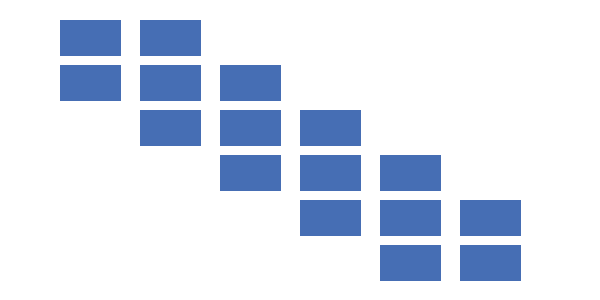
\includegraphics[width=\columnwidth]{blocks.png}
\caption{Block-sparse attention mask with $b=64$ and $g=2$.}
\label{fig:mask}
\end{figure}

\section{Experiments}
Table~\ref{tab:results} reports accuracy. Figure~\ref{fig:mask} illustrates the mask.

\begin{table}[t]
\centering
\caption{Test accuracy (\%).}
\label{tab:results}
\begin{tabular}{lccc}
\toprule
Model & Hyperpartisan & ArXiv & IMDB \\
\midrule
BERT (512)  & 87.8 & 84.1 & 93.2 \\
Longformer  & 94.8 & 86.9 & 95.7 \\
Ours        & \textbf{95.1} & \textbf{87.3} & 95.6 \\
\bottomrule
\end{tabular}
\end{table}

\begin{figure*}[t]
\centering
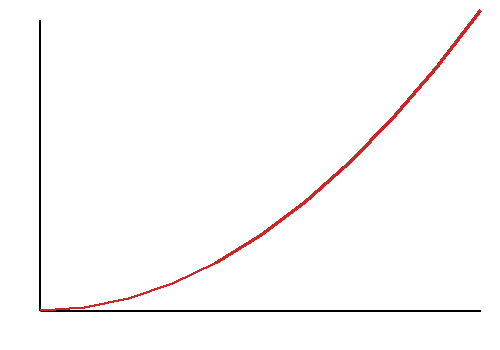
\includegraphics[width=0.8\textwidth]{plot.png}
\caption{Memory use as a function of sequence length for dense and sparse attention.}
\label{fig:memory}
\end{figure*}

\section{Conclusion}
Block-sparse attention is a simple drop-in replacement for long inputs. Code is available
at \url{https://github.com/example/sparse-attn}.

\begin{thebibliography}{1}
\bibitem{beltagy2020} I.~Beltagy, M.~E. Peters, and A.~Cohan, ``Longformer: The
long-document transformer,'' \emph{arXiv:2004.05150}, 2020.
\bibitem{zaheer2020} M.~Zaheer \emph{et~al.}, ``Big Bird: Transformers for longer
sequences,'' in \emph{NeurIPS}, 2020.
\end{thebibliography}

\end{document}
